\documentclass{beamer}
\usepackage{amsthm, multirow, hhline, graphicx, verbatim, color}
\usetheme{Ilmenau}
\usecolortheme{default}
\usepackage{caption}
\usepackage[export]{adjustbox}
\title[Biostatistics Computing Workshop]{SQL: Structured Query Language}
\author{Adam Peterson}
\date{ \\
}
\institute{University of Michigan: Department of Biostatistics
}


\begin{document}
	\begin{frame}
		\titlepage
		
		\centering
		materials found at \\
	\href{https://github.com/apeterson91/computing_workshops}{https://github.com/apeterson91/computing\_workshops/workshop\_2}
	\end{frame}

	\section{Agenda}
	\begin{frame}{Agenda}
				\begin{enumerate}
					\item Motivation
					\item Keywords:
					\begin{itemize}
						\item 'SELECT'
						\item 'WHERE'
						\item 'GROUP BY'
					\end{itemize}
					\item Inner queries
					\item Joins
					\begin{itemize}
						\item Inner
						\item Outer
						\item Left, Right
					\end{itemize}
				\end{enumerate}
	\end{frame}

	\section{Getting Started}
	\begin{frame}{Motivation}
		\begin{columns}
		\begin{column}{.5 \textwidth}
			
\includegraphics[width=1 \textwidth]{sql_image.png}
		\end{column}			
			\begin{column}{.5 \textwidth}
		\begin{itemize}
			\item What is SQL and why is it important? \pause
			\item SQL is a programming language that allows one to programmatically access data in databases \pause
			\item i.e. With SQL we can \textit{query} a database for just the information we want and nothing else.
		\end{itemize}
			\end{column}
		\end{columns}
	\end{frame}
	
	\begin{frame}{Set-Up:1 }
		\begin{minipage}{1 \textwidth}
\begin{table}[H]
	\centering
	\caption{Student\_Table}

	\begin{tabular}{|l|l|l|l|l|}
		\hline
		S\_ID & First\_Name & Last\_Name & Student\_Age & Student\_Major \\ \hline
		1           & John        & Smith      & 23           & Biostatistics  \\ \hline
		2           & Anne        & Doroughty  & 21           & Biostatistics  \\ \hline
		3           & Anthony     & Jones      & 19           & Statistics     \\ \hline
	\end{tabular}
\end{table}	
		\end{minipage}
\end{frame}

\begin{frame}{Set-Up:2}
	Loading Data into SAS for \texttt{PROC SQL} exercises
\end{frame}
	
	\section{Keywords}
	
	\subsection{SELECT Keyword}
	\begin{frame}{SELECT}
		\begin{block}{SELECT: Formulaic}
			SELECT $<$ColumnNames$>$ FROM $<$TableName$>$ 
		\end{block}
		\begin{block}{SELECT: Example}
			SELECT First\_Name FROM Student\_Table;
		\end{block}
\begin{table}[H]
	\centering
	\caption*{}

	\begin{tabular}{|l|}
		\hline
		 First\_Name  \\ \hline
			John \\ \hline
			Anne  \\ \hline
			Anthony  \\    \hline
	\end{tabular}
\end{table}			
	\end{frame}
	
	\begin{frame}{SELECT example- SAS}
		Code fairly simple... \\ \pause 
		\texttt{PROC SQL;} \\
		\texttt{SELECT First\_Name } \\
		\texttt{FROM Student\_Table;}\\
		\texttt{QUIT;}
	\end{frame}
	
	\subsection{WHERE Keyword}
	\begin{frame}{Where}
		\begin{block}{WHERE: Formulaic}
			SELECT $<$ColumnNames$>$ FROM $<$TableName$>$ 
			WHERE $<$Condition$>$
		\end{block}
		\begin{block}{WHERE: Example}
			SELECT First\_Name FROM Student\_Table 
			WHERE Student\_Age$<$22;
		\end{block}
	\begin{table}[H]
	\centering
	\caption*{}

	\begin{tabular}{|l|}
		\hline
		First\_Name  \\ \hline
		Anne  \\ \hline
		Anthony  \\    \hline
	\end{tabular}
	\end{table}		
	\end{frame}
	
	\begin{frame}{WHERE example- SAS}
		\texttt{PROC SQL;} \\
		\texttt{SELECT First\_Name } \\
		\texttt{FROM Student\_Table}\\
		\texttt{WHERE Student\_Age < 22;} 
		\texttt{QUIT;}
	\end{frame}
		\subsection{GROUP BY Keyword}
		\begin{frame}
		\begin{block}{GROUP BY: Formulaic}
			SELECT $<$ Aggregate\_Function(ColumnNames) $>$ FROM $<$TableName$>$ GROUPBY $<$GroupColumnName$>$
		\end{block}
		\begin{block}{GROUP BY: Example}
			SELECT Student\_Major, SUM(Student\_Age) FROM Student\_Table WHERE Student\_Age $>$19 GROUP BY Student\_Major;
		\end{block}
		\begin{table}[H]
			\centering
			\caption*{}

			\begin{tabular}{|l|l|}
				\hline
				Student\_Major & SUM(Student\_Age)  \\ \hline
				Biostatistics  & 44 \\ \hline
			\end{tabular}
		\end{table}			
		\end{frame}
		
	\begin{frame}{Group By example- SAS}
		\texttt{PROC SQL;} \\
		\texttt{SELECT SUM(Student\_Age) } \\
		\texttt{FROM Student\_Table}\\
		\texttt{WHERE Student\_Age > 19  } \\
		\texttt{GROUP BY Student\_Major;} \\
		\texttt{QUIT;}
	\end{frame}
	\section{Inner Queries}
	\begin{frame}
		\begin{block}{Inner Query: Formulaic}
			SELECT $<$ColumnNames$>$ FROM (SELECT $<$ColumnNames$>$ FROM $<$TableName$>$ )
		\end{block}
		\begin{block}{Inner Query: Example}
			SELECT First\_Name FROM (SELECT * FROM Student\_Table WHERE Student\_Age$<$22) ;
		\end{block}		
	\begin{table}[H]
	\centering
	\caption*{}

	\begin{tabular}{|l|}
		\hline
		First\_Name  \\ \hline
		Anne  \\ \hline
		Anthony  \\    \hline
	\end{tabular}
	\end{table}				
	\end{frame}
	
	\begin{frame}{Inner Query By example- SAS}
		\texttt{PROC SQL;} \\
		\texttt{SELECT First\_Name FROM } \\
		\texttt{(SELECT * FROM Student\_Table WHERE Student\_Age < 22) ;}\\
		\texttt{QUIT;}
	\end{frame}	
	
	
	
	\section{Joins}
	\begin{frame}{Quick Aside: Relational Databases}
		Let's talk a bit about how data is stored in tables in a relational database
		\begin{itemize}
			\item Unique Identifiers \pause
			\item One-To-Many Relationship
			\begin{itemize}
				\item One student, multiple classes \pause
			\end{itemize} 
		\end{itemize}

\begin{table}[!H]
	\centering
	\caption*{StuClass\_Table}
	\begin{tabular}{|l|l|l|l|}
		\hline
		S\_ID & Class\_Num & Class\_Name & Class\_Dept \\ \hline
		1 & 602 & Statistical Inference II & Biostatistics \\ \hline
		1 & 651 & Applied Linear Regression II & Biostatistics \\ \hline
		2 & 516 & Epidemiology II & Epidemiology \\ \hline
		3 & 601 & Statistical Inference I & Biostatistics \\ \hline
		3 & 531 & Analysis of Time Series & Statistics \\ \hline
	\end{tabular}
\end{table}

		
\end{frame}

\begin{frame}{Type of Joins}
	\begin{itemize}
		\item Left Outer
		\begin{itemize}
			\item Get everything from 'left' table, matching items from right
		\end{itemize}
		\item Right Outer
		\begin{itemize}
			\item Get everything from 'right' table, matching items from left
		\end{itemize}
		\item Inner
		\begin{itemize}
			\item  Only items that are found in both tables
		\end{itemize}
		\item More...
	\end{itemize}
\end{frame}

\begin{frame}{Type of Joins}
	\centering
	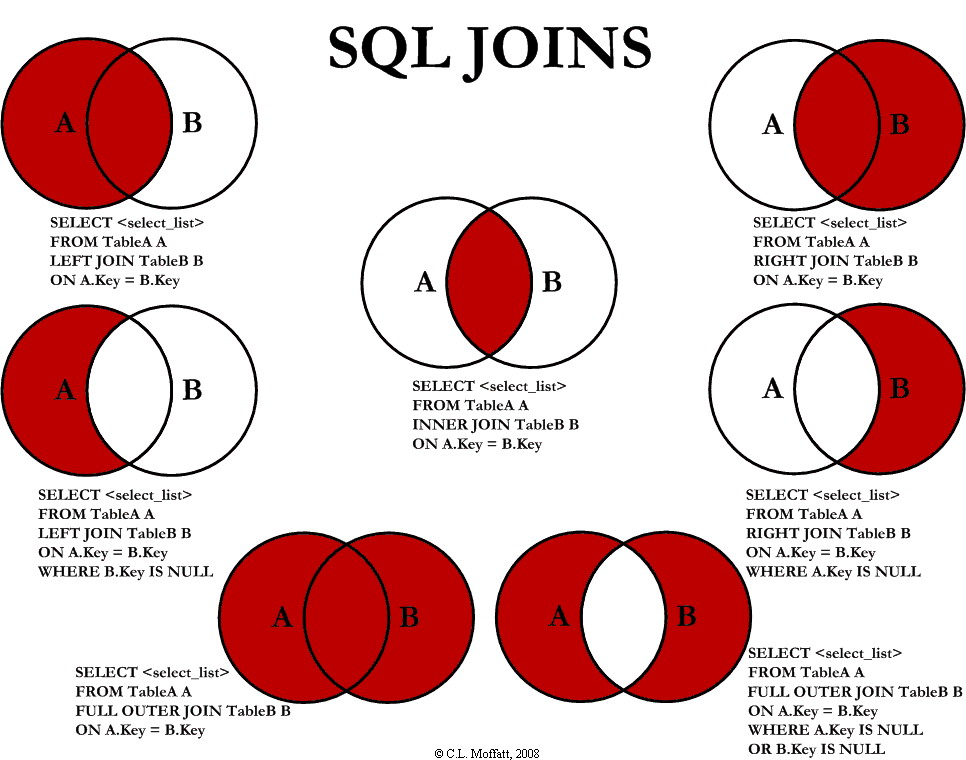
\includegraphics[width = .78 \textwidth]{Visual_SQL_JOINS_orig.jpg}
\end{frame}



	\begin{frame}{Join: Example}
		\begin{block}{Join: Formulaic}
			SELECT Table\_1.$<$ColumnNames$>$, Table\_2.$<$ColumnNames$>$ FROM $<$TableName$>$ $<$Type$>$ JOIN 
		\end{block}
		\begin{block}{Join: Example}
			SELECT Student\_Table.First\_Name StuClass\_Table.Class\_Name FROM Student\_Table INNER JOIN StuClass\_Table ON Student\_Table.S\_ID = StuClass\_Table.S\_ID;
		\end{block}	
	\end{frame}
	
	\begin{frame}{Join: Example}
			\begin{block}{Join: Example}
				SELECT Student\_Table.First\_Name, StuClass\_Table.Class\_Name FROM Student\_Table INNER JOIN StuClass\_Table ON Student\_Table.S\_ID = StuClass\_Table.S\_ID;
			\end{block}		
		\begin{table}[H]
			\centering
			\begin{tabular}{|l|l|l|}
				\hline
				Student\_ID & First\_Name & Class\_Name \\ \hline
				1 & John & Statistical Inference II \\ \hline
				1 & John & Applied Linear Regression II \\ \hline
				2 & Anne & Epidemiology II \\ \hline
				3 & Anthony & Statistical Inference I \\ \hline
				3 & Anthony & Analysis of Time Series \\ \hline
			\end{tabular}
		\end{table}
	\end{frame}
	
	\begin{frame}{SAS - Join Example}
		\texttt{PROC SQL;}\\
		\texttt{SELECT Student\_Table.First\_Name, StuClass\_Table.Class\_Name} \\
		\texttt{FROM Student\_Table}\\
		\texttt{INNER JOIN StuClass\_Table} \\
		\texttt{ON Student\_Table.S\_ID = StuClass\_Table.S\_ID ; }\\
		\texttt{QUIT;}
	\end{frame}

	\begin{frame}{R, Python and beyond}
		SQL can be found anywhere there is data:
		\begin{itemize}
			\item Server databases: Postgresql, MySQL, MS SQL Server, ...
			\item 'Local' Databases - SQLlite - cellphones, computers
		\end{itemize}
		We can query either of these using Python, R, or SAS using SQL
	\end{frame}


	\begin{frame}{Resources for Further Learning}
		\begin{itemize}
			\color{blue}
			\item \href{http://blog.yhat.com/posts/pandasql-sql-for-pandas-dataframes.html}{pandasql}
			\item \href{http://anythingbutrbitrary.blogspot.com/2012/08/manipulating-data-frames-using-sqldf.html}{sqldf}
			\item \href{https://www.codecademy.com/learn/learn-sql}{CodeAcademy's SQL Course}
			\item \href{http://www.w3schools.com/sql/}{W3} - great reference
		\end{itemize}
	\end{frame}
	
	\begin{frame}{Questions}
		\centering
		Any Questions?
	\end{frame}


\end{document}
